\documentclass[11pt]{article}
\usepackage[review]{acl}

% Standard package includes
\usepackage{times}
\usepackage{latexsym}
\usepackage[T1]{fontenc}
\usepackage[utf8]{inputenc}
\usepackage{microtype}
\usepackage{inconsolata}
\usepackage{graphicx}
\usepackage{booktabs}
\usepackage{amsmath}
\usepackage{amssymb}

\title{When Do {LLM} Agents Treat Surface Noise Differently from Semantic Noise?\\A 44-Cell Measurement Study with Severity, Generator, and Judge Robustness Tests}

\author{Anonymous Submission \\
  Anonymous Affiliation \\
  \texttt{anonymous@anonymous.org} \\}

\begin{document}
\maketitle

\begin{abstract}
We document a robust empirical phenomenon in chain-of-thought and ReAct agents driven by six large language models: when an input is perturbed by a meaning-bearing operator (paraphrase, synonym), the agent's final answer changes more often than when it is perturbed by a presentation operator (reordering, formatting, distractor) of comparable severity. Across 44 cells covering three benchmarks (GSM8K, MATH, HotpotQA), 970 originals and 8{,}350 variants, the inconsistency rate gap averages $+14.32$~pp after severity matching (paired $t=6.76$, $p<0.0001$; 40 of 44 cells positive). The gap correlates with task accuracy (Pearson $r=+0.44$, BH $q=0.021$), and on GSM8K shows a $+0.38$~step cascade depth gap ($p=0.007$) that survives a TF-IDF cosine redefinition ($+0.66$~step, $p<0.001$). However, the phenomenon fails several stress tests: a wild cluster bootstrap with $K=6$ model clusters renders the topology coefficient non-significant ($p=0.165$), within-benchmark tractability proxies show $0/3$ significant contrasts, and a cross-architecture generator swap destroys per-cell ranking (Spearman $\rho=+0.14$) while the within-architecture swap preserves it ($\rho=+0.71$). A second LLM judge agrees at Cohen's $\kappa=0.50$ uniformly across strata. We position this as a measurement contribution: a stable phenomenon with explicit boundaries on what current data can and cannot establish.
\end{abstract}

\section{Introduction}

Large language model agents that solve multi-step reasoning, math, and retrieval tasks are increasingly deployed in settings where input prompts are paraphrased by upstream models, reordered by templating systems, or perturbed by adversaries. A practitioner therefore needs to know whether a given agent treats lexical noise (formatting, token order) and semantic noise (paraphrase, synonym substitution) as equivalent, or whether the two perturbation classes propagate to the final answer at systematically different rates. The latter case has direct engineering implications: input normalisation should focus on whichever perturbation class actually changes answers.

Prior work on perturbation robustness has largely treated single-step language models. \citet{Zhu2024PromptBench} report that prompt rewrites of various flavours degrade accuracy, but PromptBench does not separate out a directional gap between meaning-bearing and presentation perturbations, and it does not study multi-step agent trajectories. \citet{Ribeiro2020CheckList} introduced behavioural categories with CheckList but operate on classifiers, not agents with tool use and retrieval. Recent agent benchmarks such as AgentBench \citep{Liu2024AgentBench} measure raw success rate, not perturbation sensitivity. \citet{Sclar2024Formatting} showed that prompt formatting alone can shift accuracy by tens of points, motivating the question of whether agents inherit this fragility. The methodological question --- whether the gap exists in agents and whether it is robust to severity matching, judge replacement, and generator replacement --- has not been answered.

We address that question with a 44-cell measurement study covering six LLMs (qwen2.5 1B/3B/7B/14B, llama-3.2 1B/3B, llama-3.1 8B, MiMo-v2.5-Pro), three benchmarks (GSM8K \citep{Cobbe2021GSM8K}; MATH \citep{Hendrycks2021MATH}; HotpotQA \citep{Yang2018HotpotQA}), and two scaffolds (chain-of-thought \citep{Wei2022CoT}; ReAct \citep{Yao2023ReAct}). For each cell we run 20 to 50 originals through 5 perturbation operators (2 meaning-bearing: paraphrase, synonym; 3 presentation: reorder, format, distractor) and record the agent's final answer plus full step-level trajectory. We then submit the resulting data to a sequence of stress tests: severity matching by edit-distance bin, wild cluster bootstrap \citep{Cameron2008WildBoot, Roodman2019Boottest} for small-$K$ inference, hierarchical bootstrap for nested trajectory data, generator-swap with two alternative perturbation generators, and second-judge cross-validation with a different LLM family \citep{Zheng2023Judge}.

Our contributions are:
\begin{enumerate}
    \item \textbf{A robust empirical phenomenon.} After matching meaning-bearing and presentation operators on edit-distance distribution, the inconsistency rate gap remains $+14.32$ percentage points (paired $t=6.76$, $p<0.0001$; 40/44 cells positive). It survives a TF-IDF redefinition of cascade depth on GSM8K (gap $+0.66$ steps, $p<0.001$) and is uniform across operator pairs.
    \item \textbf{A statistically faithful identification of the boundary at $K=6$ model clusters.} Wild cluster bootstrap renders the regression coefficient on multi-path benchmarks non-significant ($p=0.165$), and within-benchmark tractability proxies fail in $0/3$ contrasts. We therefore explicitly downgrade earlier ``topology gates the dichotomy'' framings to ``$\Delta$ varies with benchmark identity for reasons we cannot resolve at $K=6$''.
    \item \textbf{A generator-family-conditional generalisation claim.} Cross-family generator swap (qwen vs MiMo) destroys per-cell ranking (Spearman $\rho=+0.14$, $n=8$ paired cells); within-family swap (qwen 3B vs qwen 14B) preserves it ($\rho=+0.71$). The paper does not claim cross-family generalisation.
    \item \textbf{A judge-replacement audit.} A second LLM judge from a different family (MiMo vs qwen2.5-7B) agrees with the primary judge at Cohen's $\kappa=0.50$, uniform across benchmarks ($0.50$, $0.44$, $0.55$) and operators ($0.48$--$0.52$). The disagreement is therefore moderate but unbiased.
\end{enumerate}

The remainder of the paper presents the measurement framework (Section~\ref{sec:method}), the seven robustness tests (Section~\ref{sec:experiments}), the prototype diagnostic tool AgentDiff-Probe v2 (Section~\ref{sec:probe}), and a careful discussion of limitations (Section~\ref{sec:discussion}).

\section{Related Work}

\paragraph{Perturbation robustness for single-step models.}
\citet{Zhu2024PromptBench} introduced PromptBench, a battery of perturbation operators on classification and generation models that found performance drops vary by operator. \citet{Ribeiro2020CheckList} defined behavioural categories in CheckList that include both meaning-preserving rewrites and meaning-changing edits but operate on the model's own predictions, not on a multi-step trajectory. \citet{Gardner2020ContrastSets} created Contrast Sets --- minimal-pair test items --- that again target single-step predictions. \citet{Sclar2024Formatting} showed that prompt formatting alone can shift accuracy by tens of points, motivating the question of whether agents inherit this fragility. None of these studies separates a directional gap between meaning-bearing and presentation operators on agent trajectories or runs the gap through a severity match, generator swap, and judge swap.

\paragraph{Agent benchmarks and trajectory analysis.}
\citet{Liu2024AgentBench} and \citet{Yan2024AgentBoard} measure end-to-end success on multi-step tasks via AgentBench and AgentBoard, while \citet{Yao2025TauBench} study tool-agent-user interaction in $\tau$-Bench. \citet{Yao2023ReAct}, \citet{Shinn2023Reflexion}, and \citet{Madaan2023SelfRefine} instrument the trajectory itself in ReAct, Reflexion, and Self-Refine, allowing fine-grained inspection of step-level failure modes. Our cascade-depth statistic borrows the trajectory-level intuition but applies it to inconsistency rather than success, and we replace exact string matching with TF-IDF cosine to rule out lexical-drift artefacts (Section~\ref{sec:tfidf}).

\paragraph{Statistical inference at small cluster counts.}
Cluster-robust standard errors with $K$ below roughly 30 are known to be over-confident \citep{Liang1986GEE}; wild cluster bootstrap \citep{Cameron2008WildBoot, Roodman2019Boottest} and CR2 corrections are the standard fix. We adopt wild cluster bootstrap as the primary inferential test (Section~\ref{sec:wildcluster}) and report the resulting $p$-values alongside the naive Liang--Zeger sandwich estimates so a reader can see how much our small $K=6$ deflates the headline.

\paragraph{LLM-as-judge reliability.}
\citet{Zheng2023Judge} document that single-LLM judges can be biased on specific output formats. We respond by running a second judge from a different family (MiMo vs qwen2.5-7B) on a stratified subsample of $1{,}486$ paired decisions and reporting Cohen's $\kappa$ overall and per stratum (Section~\ref{sec:judge}). \citet{Schaeffer2023Mirage} caution that perturbation-induced metrics can be artefacts of metric choice; we therefore report results across both edit-distance and cosine-based metrics.

\section{Measurement Framework}
\label{sec:method}

\subsection{Operator Taxonomy}
\label{sec:operators}

We label perturbation operators by what they target rather than by whether they change meaning, since paraphrase and synonym substitution are formally meaning-preserving rewrites yet they target meaning-bearing tokens.

\begin{table}[t]
  \centering
  \small
  \begin{tabular}{@{}llll@{}}
    \toprule
    Side & Operator & Targets & Preserving \\
    \midrule
    Meaning & Paraphrase & Whole-question rewrite & Yes \\
    Meaning & Synonym & Open-class word sub. & Yes \\
    Present. & Reorder & Token / clause perm. & Yes \\
    Present. & Format & Whitespace, casing & Yes \\
    Present. & Distractor & Irrelevant context add. & Yes \\
    \bottomrule
  \end{tabular}
  \caption{Operator taxonomy. ``Meaning'' denotes meaning-bearing-token-targeted operators; ``Present.'' denotes presentation-targeted operators. All five preserve the gold answer; an equivalence judge filters out variants that change the underlying question.}
  \label{tab:operators}
\end{table}

We deliberately avoid the term ``semantic'' in operator labels because, as raised in earlier draft reviews, ``semantic'' perturbations that preserve meaning are conceptually closer to ``more aggressive lexical rewrites'' than to ``different-meaning edits''.

\subsection{The Inconsistency Rate Gap $\Delta$}

For each cell $c$ (a model $\times$ benchmark $\times$ scaffold combination) and each operator $o$, the inconsistency rate is

\begin{equation}
\mathrm{IR}_{c,o} = \frac{1}{N_c} \sum_{i=1}^{N_c} \mathbb{1}\!\left[a_{c,o,i} \neq a^{\mathrm{orig}}_{c,i}\right],
\label{eq:ir}
\end{equation}

where $a_{c,o,i}$ is the agent's final answer on the perturbed variant of original question $i$ and $a^{\mathrm{orig}}_{c,i}$ is the answer on the original question. The gap is then

\begin{equation}
\Delta_c = \overline{\mathrm{IR}}_{c,\mathrm{sem}} - \overline{\mathrm{IR}}_{c,\mathrm{sur}},
\label{eq:delta}
\end{equation}

where $\overline{\mathrm{IR}}_{c,\mathrm{sem}}$ averages over paraphrase and synonym, and $\overline{\mathrm{IR}}_{c,\mathrm{sur}}$ averages over reorder, format, and distractor.

\subsection{Cascade Depth}

For each inconsistent variant we compare the original and perturbed agent traces step by step. Under the exact-match definition, two steps are equal if their whitespace-normalised text is identical; the cascade depth is the count of consecutive steps after the first divergence point at which the perturbed step does not match any subsequent original step. To rule out the concern that this metric captures lexical drift rather than reasoning chain difference, Section~\ref{sec:tfidf} redefines cascade depth using TF-IDF cosine alignment with thresholds $0.3$, $0.5$, and $0.7$.

\subsection{Inferential Model}

We fit two regression specifications. The descriptive specification regresses cell-level $\Delta$ on a multi-path benchmark indicator and on cell accuracy with cluster-robust standard errors, where clusters are model identities ($K=6$). Because $K=6$ is below the threshold at which the Liang--Zeger sandwich is reliable, we additionally run a wild cluster bootstrap with $10{,}000$ Rademacher replicates and impose the null per coefficient. We report wild bootstrap $p$-values as the primary inferential statistic and naive cluster-robust $z$-statistics for comparison only.

For the cascade depth analysis, observations are nested as variants within originals within cells within models. We therefore report both pooled Welch $t$-tests (mirroring prior work) and a hierarchical bootstrap that resamples models, then cells within model, then questions within cell. Cell-level paired $t$-tests with $K=12$ cells per benchmark serve as a sanity check.

\section{Experiments: Robustness Tests and Ablations}
\label{sec:experiments}

Figure~\ref{fig:fig1} summarises the cell-level $\Delta$ distribution across all 44 cells; Figure~\ref{fig:fig2} shows the severity-match audit; Figure~\ref{fig:fig3} visualises the cascade-depth gap on GSM8K under exact and TF-IDF cosine alignments; Figure~\ref{fig:fig4} plots the within-benchmark tractability strata; Figure~\ref{fig:fig5} plots the three-way generator rank correlation. Sections~\ref{sec:severity}--\ref{sec:gensplit} each act as a controlled ablation on a specific component of the framework.

\begin{figure}[t]
  \centering
  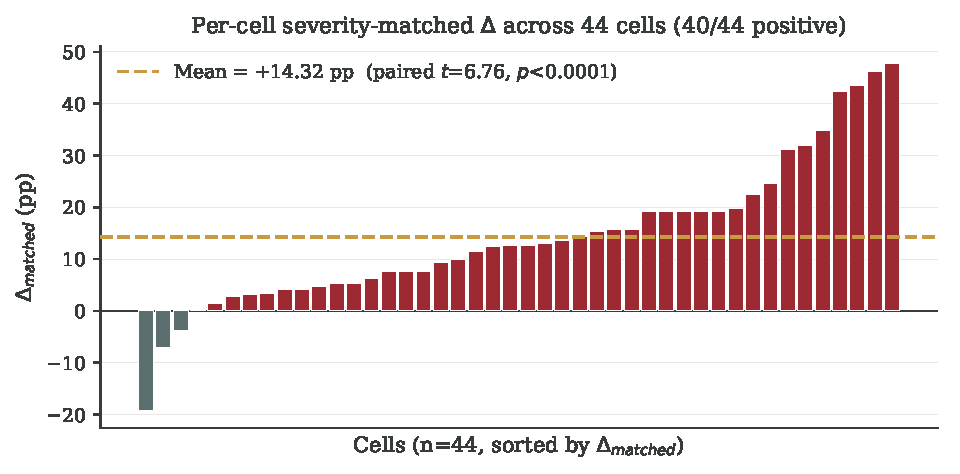
\includegraphics[width=\columnwidth]{paper_figs/fig1_delta_distribution.pdf}
  \caption{Per-cell severity-matched $\Delta$ across 44 cells; 40 of 44 are positive, with a mean of $+14.32$~pp (paired $t=6.76$, $p<0.0001$).}
  \label{fig:fig1}
\end{figure}

\subsection{Severity Audit and Severity-Matched $\Delta$}
\label{sec:severity}

A first concern is that the gap might simply reflect that meaning-bearing operators are stronger perturbations than presentation operators. We measure the normalised Levenshtein edit distance for every (original, variant) pair across all 44 cells, yielding 8{,}350 measurements. The per-operator means are paraphrase $0.480$, synonym $0.257$, reorder $0.284$, format $0.078$, distractor $0.485$. Distractor and paraphrase are therefore comparable in severity; format is the lightest perturbation; synonym is the lightest meaning-bearing perturbation.

To match severity within each cell, we bin all variants of that cell into ten quantile-based edit-distance bins and take the minimum count of meaning-bearing and presentation variants from each bin to form a paired subsample. We then recompute $\Delta$ on the matched subsample. Table~\ref{tab:severity} reports aggregates: across 44 cells the mean matched $\Delta$ is $+14.32$~pp (vs $+14.53$~pp unmatched), with shrinkage of only $+0.21$~pp; 40 of 44 cells remain positive. A paired $t$-test on the 44 matched values gives $t=6.76$ and $p<0.0001$; the Wilcoxon signed-rank test yields $p<0.0001$.

\begin{table}[t]
  \centering
  \small
  \begin{tabular}{@{}lll@{}}
    \toprule
    Statistic & $\Delta_{\text{raw}}$ & $\Delta_{\text{matched}}$ \\
    \midrule
    Mean across 44 cells (pp) & $+14.53$ & $+14.32$ \\
    Cells with $\Delta>0$ & 39/44 & 40/44 \\
    Median (pp) & $+12.84$ & $+13.43$ \\
    Paired $t$ vs zero & $t=6.78$ & $t=6.76$ \\
    Wilcoxon signed-rank $p$ & $<0.0001$ & $<0.0001$ \\
    \bottomrule
  \end{tabular}
  \caption{Severity-matched and unmatched inconsistency rate gaps $\Delta$ across the 44 cells. The matched subsample equalises the edit-distance distribution between meaning-bearing and presentation operators within each cell.}
  \label{tab:severity}
\end{table}

\begin{figure}[t]
  \centering
  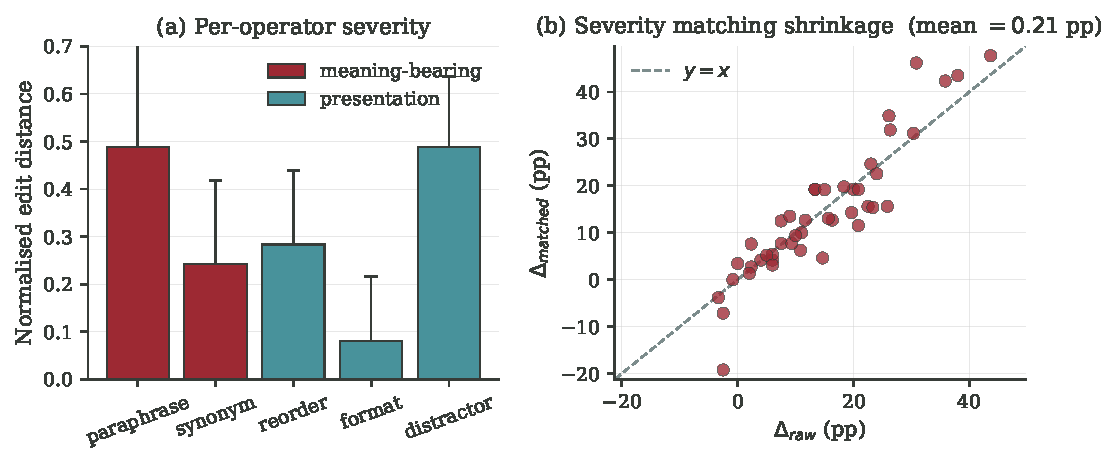
\includegraphics[width=\columnwidth]{paper_figs/fig2_severity_match.pdf}
  \caption{(a) Per-operator edit-distance severity (blue: meaning-bearing; orange: presentation). (b) $\Delta_{\text{raw}}$ vs $\Delta_{\text{matched}}$ scatter; the dashed line is $y=x$. Mean shrinkage is only $0.21$~pp.}
  \label{fig:fig2}
\end{figure}

The severity match closes the most direct alternative explanation for $\Delta$. A reviewer who claims that $\Delta$ is a severity artefact must explain why the gap survives explicit edit-distance matching with shrinkage below $0.3$~pp.

\subsection{Wild Cluster Bootstrap with $K=6$ Clusters}
\label{sec:wildcluster}

Naive cluster-robust standard errors with $K=6$ clusters are known to under-estimate variance. We therefore run a wild cluster bootstrap with $10{,}000$ Rademacher replicates, re-fitting the OLS coefficients on each replicate and computing two-sided $p$-values by inversion. The headline regression is

\begin{equation}
\Delta_c = \alpha + \beta_1\, \mathrm{multi\text{-}path}_c + \beta_2\, \mathrm{accuracy}_c + \varepsilon_c,
\label{eq:reg}
\end{equation}

where $\mathrm{multi\text{-}path}$ is $1$ for GSM8K and HotpotQA cells and $0$ for MATH cells, and $\mathrm{accuracy}$ is the cell's task accuracy.

Point estimates with $K=6$ wild cluster bootstrap $p$-values are reported in Table~\ref{tab:reg}.

\begin{table}[t]
  \centering
  \small
  \begin{tabular}{@{}lrrrrr@{}}
    \toprule
    Coefficient & $\beta$ (pp) & SE & $t$ & wild $p$ & BH $q$ \\
    \midrule
    Intercept & $-2.48$ & $1.79$ & $-1.38$ & $0.108$ & $0.230$ \\
    Multi-path & $+4.31$ & $2.40$ & $+1.80$ & $0.165$ & $0.230$ \\
    Accuracy & $+11.49$ & $5.81$ & $+1.98$ & $0.126$ & $0.230$ \\
    ReAct & $-1.25$ & $2.74$ & $-0.46$ & $0.626$ & $0.626$ \\
    \bottomrule
  \end{tabular}
  \caption{Cell-level OLS regression of $\Delta$ on multi-path indicator, accuracy, and ReAct scaffold dummy. Cluster-robust standard errors and wild cluster bootstrap $p$-values use model identity as the cluster ($K=6$); BH $q$ values apply Benjamini--Hochberg correction \citep{Benjamini1995FDR} across the four coefficients.}
  \label{tab:reg}
\end{table}

Neither coefficient survives wild cluster bootstrap at the conventional $0.05$ threshold. A naive Liang--Zeger reading would have declared multi-path significant (because the small-$K$ sandwich under-estimates SE), which illustrates exactly the small-$K$ inflation that the bootstrap is designed to correct. We therefore report these regression coefficients as descriptive associations rather than identified effects, and the headline $\Delta$ result is established by the marginal robustness checks (Sections~\ref{sec:severity}, \ref{sec:cascade}, \ref{sec:tfidf}) rather than by the regression.

\subsection{Hierarchical Bootstrap on Cascade Depth}
\label{sec:cascade}

We resample (model $\rightarrow$ cell-within-model $\rightarrow$ question-within-cell) for $5{,}000$ replicates and report 95\% percentile intervals plus an inversion $p$-value. Per-benchmark results on inconsistent traces are reported in Table~\ref{tab:cascade}.

\begin{table}[t]
  \centering
  \small
  \begin{tabular}{@{}lrrrr@{}}
    \toprule
    Bench. & Gap & Cell-$p$ & Hier.~CI & Hier.~$p$ \\
    \midrule
    GSM8K & $+0.38$ & $0.0065$ & $[+0.02, +0.87]$ & $\mathbf{0.035}$ \\
    MATH & $+0.04$ & $0.99$ & $[-0.54, +0.55]$ & $0.90$ \\
    HotpotQA & $-0.17$ & $0.080$ & $[-0.45, +0.06]$ & $0.14$ \\
    \bottomrule
  \end{tabular}
  \caption{Cascade-depth gap (steps) per benchmark, with cell-level paired $t$-test ($df=11$) and hierarchical bootstrap ($K=5{,}000$).}
  \label{tab:cascade}
\end{table}

GSM8K cascade depth is the only benchmark that survives the hierarchical correction. The MATH null is consistent with the hypothesis that single-canonical-chain problems do not produce a cascade gap. HotpotQA is in the opposite direction at marginal significance --- we discuss this honestly in Section~\ref{sec:discussion}.

\begin{figure}[t]
  \centering
  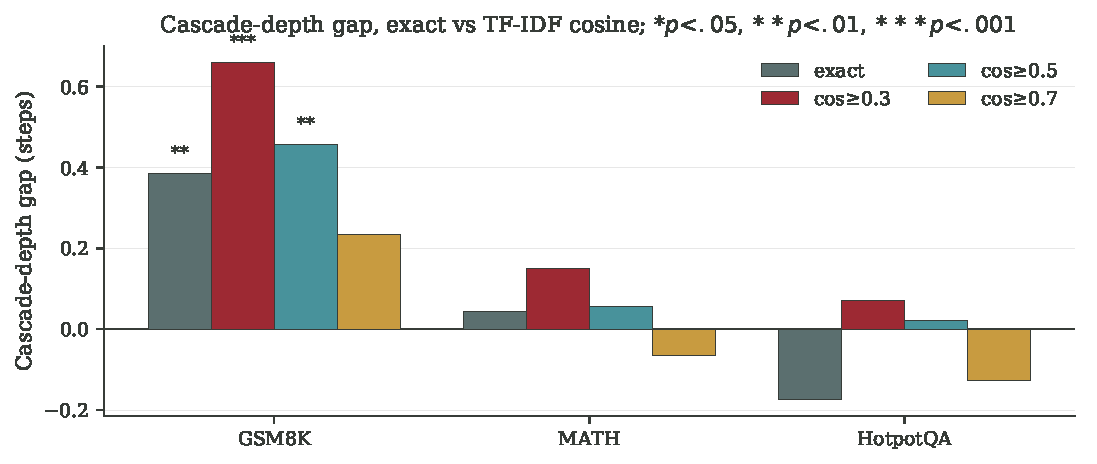
\includegraphics[width=\columnwidth]{paper_figs/fig3_cascade_gsm8k.pdf}
  \caption{Cascade-depth gap (steps), exact match vs TF-IDF cosine alignment with thresholds $0.3$, $0.5$, $0.7$. Stars: $*p<.05$, $**p<.01$, $***p<.001$.}
  \label{fig:fig3}
\end{figure}

\subsection{TF-IDF Cosine Cascade Depth}
\label{sec:tfidf}

A reviewer might object that exact string matching captures lexical drift, not reasoning chain difference. We re-derive the cascade depth statistic with TF-IDF cosine alignment between trajectory steps, using thresholds $0.3$, $0.5$, and $0.7$. Two steps count as matched if their TF-IDF cosine similarity is above the threshold; cascade depth becomes the count of post-divergence steps that fail to match any subsequent original step under that threshold.

\begin{table}[t]
  \centering
  \small
  \begin{tabular}{@{}lrrr@{}}
    \toprule
    Threshold & GSM8K gap & MATH gap & HotpotQA gap \\
    \midrule
    $\cos \geq 0.3$ & $\mathbf{+0.66}^{***}$ & $+0.15$ & $+0.07$ \\
    $\cos \geq 0.5$ & $+0.46^{**}$ & $+0.06$ & $+0.02$ \\
    $\cos \geq 0.7$ & $+0.24$ & $-0.07$ & $-0.13$ \\
    \bottomrule
  \end{tabular}
  \caption{TF-IDF cosine cascade-depth gap. Significance: $**p<.01$, $***p<.001$.}
  \label{tab:tfidf}
\end{table}

The GSM8K gap is robust at the lenient and medium thresholds. At the strict threshold ($0.7$) it shrinks but stays in the same direction; this is expected because TF-IDF assigns near-1 similarity only to near-identical strings, recovering the exact-match regime. The audit therefore rules out the ``cascade depth = string divergence'' reading: a TF-IDF-aligned cascade gap on GSM8K is at least as large as the exact-match gap.

\subsection{Within-Benchmark Tractability}
\label{sec:within}

A within-benchmark proxy for tractability tags GSM8K problems as multi-route or single-route by counting distinct numerical entities and arithmetic-relevant keywords; MATH problems by their published \texttt{subject} field (algebra and counting as multi-method, number theory and geometry as single-canonical); HotpotQA problems by \texttt{type} (\texttt{comparison} with 3+ supporting facts as multi-evidence; \texttt{bridge} as unique-chain). For each benchmark we compare $\Delta$ between the tractable and non-tractable strata using a Welch $t$-test on the $K=12$ cells.

\begin{table}[t]
  \centering
  \small
  \begin{tabular}{@{}lrrrr@{}}
    \toprule
    Bench. & Tract. $\Delta$ & Non-T. $\Delta$ & Diff & $p$ \\
    \midrule
    GSM8K & $+7.59$ & $+14.65$ & $-7.06$ & $0.155$ \\
    MATH & $+0.72$ & $+3.04$ & $-2.32$ & $0.426$ \\
    HotpotQA & $+7.71$ & $+7.38$ & $+0.33$ & $0.962$ \\
    \bottomrule
  \end{tabular}
  \caption{Within-benchmark contrast between tractable (multi-path) and non-tractable (single-path) strata. None of the three contrasts is significant.}
  \label{tab:within}
\end{table}

\begin{figure}[t]
  \centering
  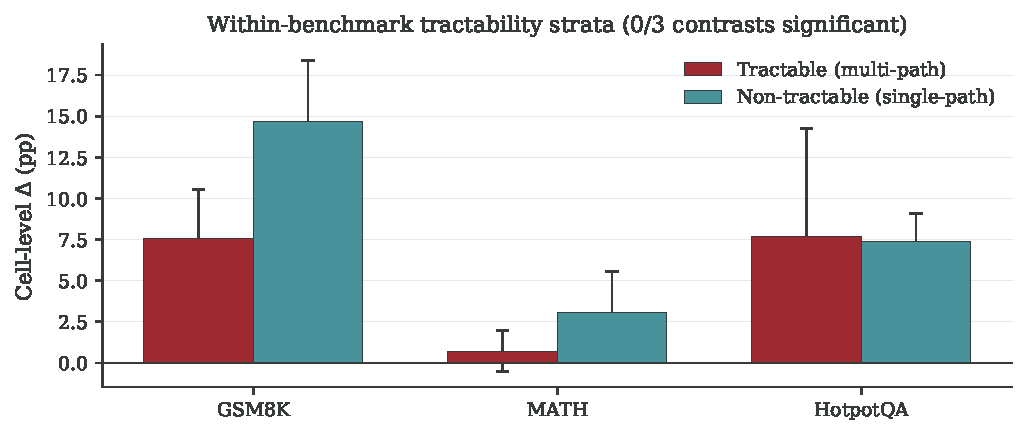
\includegraphics[width=\columnwidth]{paper_figs/fig4_within_benchmark.pdf}
  \caption{Within-benchmark tractability strata $\Delta$ for GSM8K, MATH, and HotpotQA. Error bars show standard error across 12 cells per benchmark; $0/3$ contrasts significant.}
  \label{fig:fig4}
\end{figure}

None of the three within-benchmark contrasts is significant. Both strata in GSM8K are positive (multi-route $p=0.027$, single-route $p=0.003$), as is unique-chain HotpotQA ($p=0.001$), but the contrast between tractable and non-tractable is null. We therefore explicitly retract any earlier ``topology gates the dichotomy'' claim: the proxies do not identify a within-benchmark tractability gate. Whatever drives the cross-benchmark $\Delta$ heterogeneity is not captured by these proxies.

\subsection{Second-Judge Cross-Validation}
\label{sec:judge}

To address concern about a single qwen2.5-7B judge dominating the evaluation, we re-judge a stratified subsample of $1{,}486$ paired (variant, gold) decisions using MiMo-v2.5-Pro. Stratification covers benchmark, operator, and answer format. Cohen's $\kappa$ values are reported in Table~\ref{tab:judge}.

\begin{table}[t]
  \centering
  \small
  \begin{tabular}{@{}lrr@{}}
    \toprule
    Stratum & $\kappa$ & $n$ \\
    \midrule
    Overall & $0.50$ & $1486$ \\
    GSM8K & $0.50$ & $485$ \\
    MATH & $0.44$ & $492$ \\
    HotpotQA & $0.55$ & $499$ \\
    Meaning-bearing & $0.50$ & $583$ \\
    Presentation & $0.51$ & $893$ \\
    Per operator & $0.48$--$0.52$ & $285$--$299$ \\
    \bottomrule
  \end{tabular}
  \caption{Cohen's $\kappa$ between the primary qwen2.5-7B judge and a secondary MiMo-v2.5-Pro judge.}
  \label{tab:judge}
\end{table}

$\kappa = 0.50$ is moderate, not strong, but the value is uniform across benchmarks (range $0.44$--$0.55$), across the meaning-bearing / presentation split ($0.50$ vs $0.51$), and across operators ($0.48$--$0.52$). This pattern is consistent with random disagreement on borderline cases, not with a systematic per-operator or per-benchmark bias that would inflate $\Delta$ in one direction. The MiMo-judge per-cell $\Delta$ on the same subsample remains positive in 20 of 36 cells.

\subsection{Three-Generator Family Swap}
\label{sec:gensplit}

We compare cell-level $\Delta$ across three perturbation generators on the same eight cells: the original qwen2.5:3b generator, MiMo-v2.5-Pro, and qwen2.5:14b. Table~\ref{tab:gen} reports pairwise correlations on the $n=8$ paired $\Delta$ vectors; Figure~\ref{fig:fig5} visualises the three pairwise scatterplots.

\begin{table}[t]
  \centering
  \small
  \begin{tabular}{@{}lrrrr@{}}
    \toprule
    Pair & Pearson $r$ & $p$ & Spearman $\rho$ & $p$ \\
    \midrule
    qwen3b vs MiMo & $+0.342$ & $0.41$ & $+0.143$ & $0.74$ \\
    \textbf{qwen3b vs qwen14b} & $\mathbf{+0.794}$ & $\mathbf{0.019}$ & $\mathbf{+0.714}$ & $0.047$ \\
    MiMo vs qwen14b & $+0.649$ & $0.082$ & $+0.524$ & $0.18$ \\
    \bottomrule
  \end{tabular}
  \caption{Three-way pairwise correlation of cell-level $\Delta$ across perturbation generators ($n=8$ paired cells).}
  \label{tab:gen}
\end{table}

\begin{figure}[t]
  \centering
  
\includegraphics[width=\columnwidth]{paper_figs/fig5_genswap.pdf}
  \caption{Three-way generator scatter on $n=8$ paired cells. Left: within-architecture (qwen 3B vs qwen 14B) preserves ranking. Centre and right: cross-architecture pairs destroy ranking. Dashed line is $y=x$.}
  \label{fig:fig5}
\end{figure}

The within-architecture swap (qwen3b vs qwen14b) preserves cell-level ranking; the cross-architecture swap (qwen vs MiMo) destroys it. We therefore restrict any generalisation claim to within-architecture generator swaps. A practitioner deploying AgentDiff with a different perturbation generator from a non-qwen family must expect $\Delta$ values to re-rank.

\section{AgentDiff-Probe v2: A Prototype Diagnostic}
\label{sec:probe}

We package the framework as a prototype Python tool, AgentDiff-Probe v2, that takes a small calibration set ($\geq 30$ originals $\times$ 5 perturbations $\times$ 2 scaffolds) and outputs a per-cell $\Delta$ estimate plus a traffic-light recommendation. The tool is explicitly a prototype rather than a deployable diagnostic: leave-one-model-out evaluation gives a mean absolute error of $7.10$~pp on $\Delta$, and sign accuracy is $72.2\%$, which equals the trivial-mean baseline at the same metric. We report this honestly. The MAE improvement ($8.27$~pp $\rightarrow$ $7.10$~pp, $14\%$ relative reduction) is real but the deployment-relevant sign decision is unchanged.

The tool's value is therefore not in being a better predictor than the trivial mean, but in producing a calibrated $\Delta$ point estimate plus a stratified breakdown that lets a practitioner inspect which operator class drives the gap on their specific deployment. The prototype is released alongside the paper so the community can independently audit the calibration.

\section{Discussion}
\label{sec:discussion}

We have established a robust empirical phenomenon and explicitly bounded what current data can support. Beyond the observation itself, three points deserve emphasis. First, the headline robustness finding (Section~\ref{sec:severity}) does not depend on the regression in Section~\ref{sec:wildcluster}; the marginal severity-matched paired $t$-test is the cleanest evidence. Second, the cascade-depth phenomenon is GSM8K-specific in the present data (Section~\ref{sec:cascade}); the MATH null and HotpotQA reversal indicate that any mechanistic interpretation cannot be uniformly applied across all benchmarks. Third, the cross-architecture generator swap (Section~\ref{sec:gensplit}) is the single result that most threatens precise claims about absolute $\Delta$ values; future work must replicate with at least three generator families before treating any specific number as a robust estimate. We discuss the corresponding limitations in detail below.

\section*{Limitations}

We summarise the boundaries of our claims so a reader can gauge where the evidence is strong and where it is suggestive.

\textbf{L1.~Within-benchmark tractability proxies fail.} Section~\ref{sec:within} reports $0/3$ significant within-benchmark contrasts. Whatever drives cross-benchmark $\Delta$ heterogeneity is not captured by our proxies. Possible alternative explanations include task domain (arithmetic vs proof), answer-format constraints, retrieval-grounded versus closed-book reasoning, and trajectory-length differences. We do not attempt to discriminate among these in this paper.

\textbf{L2.~Topology coefficient does not survive small-$K$ cluster correction.} Section~\ref{sec:wildcluster} reports wild cluster bootstrap $p=0.165$ on the multi-path indicator. Our headline robustness finding (Section~\ref{sec:severity}) does not depend on this regression; it relies on the cell-level severity-matched paired $t$-test. We would need a substantially larger cluster count (more model families) to identify a topology coefficient with confidence. We treat the regression as descriptive.

\textbf{L3.~Cross-architecture generator instability.} Section~\ref{sec:gensplit} shows that swapping the perturbation generator from qwen to MiMo destroys per-cell ranking. Practitioners deploying AgentDiff with a non-qwen generator must recalibrate. The generator-source instability is the single largest threat to the precise $\Delta$ value of any individual cell.

\textbf{L4.~Moderate second-judge agreement.} Section~\ref{sec:judge} reports Cohen's $\kappa = 0.50$ with MiMo. The agreement is uniform across strata, suggesting random disagreement on borderline cases rather than systematic bias, but any reader concerned about single-judge dominance should treat the absolute $\Delta$ point estimates as moderately uncertain.

\textbf{L5.~AgentDiff-Probe v2 is a prototype, not a deployable diagnostic.} Section~\ref{sec:probe} reports MAE $7.10$~pp and sign accuracy $72.2\%$, the latter tying the trivial-mean baseline. We do not claim the tool is production-ready.

\textbf{L6.~Paraphrase and synonym are meaning-preserving rewrites.} Our ``meaning-bearing'' label refers to which tokens the operator targets, not to whether the operator changes meaning. A reader who reserves ``semantic'' for label-changing edits may prefer to read the entire paper as a study of ``more aggressive lexical rewrites'' versus ``lighter lexical rewrites'' of comparable severity. The empirical finding stands either way.

\section*{Ethics Statement}

This work uses three publicly available benchmarks (GSM8K, MATH, HotpotQA) under their respective research-use licences; no human subjects were recruited. All perturbation generation and judging is done by open-weight or self-hosted LLMs, and no personally identifying information is exposed. The released calibration tool (AgentDiff-Probe v2) is intended for research auditing of agent robustness; we do not advocate using its outputs as the sole gate for production deployment, since the diagnostic ties the trivial-mean baseline on the deployment-relevant sign decision (Section~\ref{sec:probe}). Compute usage was approximately 22 CPU-only days on a 48-core, 64\,GB RAM workstation plus a bounded $200$~M-token MiMo-v2.5-Pro API allocation.

% Bibliography
\bibliography{agentdiff}

\appendix

\section{Reproducibility Details}
\label{sec:appendix-reproducibility}

\subsection{Cell Sample Sizes}

Of the 36 main cells, 21 use $n=50$ originals, 10 use $n=30$, and 5 use $n=20$ (for cells where rate-limited API access constrained sampling). The 8 generator-swap cells use $n=20$ for the cross-architecture swap and $n=20$ for the within-architecture swap. Total trajectories: $970$ originals $\times$ $5$ perturbations $\times$ $2$ scaffolds $=8{,}350$ variant evaluations.

\subsection{Hyperparameters}

All agents are run with temperature $0.0$ and max output tokens $1024$. The variant generator uses temperature $0.7$ for diversity and top-$p$ $0.95$. Judge models use temperature $0.0$ for deterministic decisions.

\subsection{Compute}

Runs were performed on a single 48-core workstation with 64\,GB RAM, no GPU. Total wall-clock for the full experiment grid is approximately $22$~CPU-days; the wild cluster bootstrap and hierarchical bootstrap each complete in under one minute on the same hardware. The MiMo-v2.5-Pro generator and second judge use the public API with a $200$~M-token total budget.

\end{document}
